\section{System Design}
\label{sec:systemdesign}

This chapter describes the system design and pre-development phase of the work, focusing on architectural decisions, platform constraints, and prototyping strategy. The target platform is the Apple Vision Pro (AVP), developed under the standard Apple Developer Program (ADP). In this configuration, critical entitlements such as direct access to raw camera frames and inertial measurement unit (IMU) data are restricted and reserved for the Apple Vision Pro program with extended entitlements (ADEP).

These limitations drive the overall architecture. Instead of streaming sensor data directly from the headset, an AirPlay-based mirroring approach is used to obtain RGB frames externally, while the VisionOS client focuses on interaction, configuration, and visualization. A Python-based backend orchestrates a computer vision pipeline and forwards prepared inputs to a FoundationPose-based 6D pose estimation API.

Before implementing the full AR interface on the AVP, two prototyping stages were carried out, summarized in Table~\ref{tab:prototyping-stages}.

\begin{table}[H]
    \centering
    \caption{Pre-development prototyping stages}
    \label{tab:prototyping-stages}
    \begin{tabular}{p{0.25\linewidth}p{0.65\linewidth}}
        \toprule
        \textbf{Prototype} & \textbf{Purpose} \\
        \midrule
        Web prototype (HTML/CSS/JS) &
        Validate ROI interaction concepts, color-based mask extraction, and basic UI layouts in a fast iteration loop. \\
        Python desktop prototype &
        Explore intrinsics estimation, depth estimation strategies, concurrency, and integration with mock and real pose APIs in a fully controllable environment. \\
        \bottomrule
    \end{tabular}
\end{table}

The remainder of this chapter describes the overall architecture, the main API and pose backend, the computer vision pipeline, the Python prototype, and the AR interface design. Occlusion-aware pose correction strategies are summarized at the end and detailed further in Appendix~\ref{appendix:willems}.

\subsection{System Overview}

Figure~\ref{fig:sysdesign} shows the high-level system architecture. The system consists of four main components, summarized in Table~\ref{tab:system-components}.

\begin{table}[H]
    \centering
    \caption{Main system components}
    \label{tab:system-components}
    \begin{tabular}{p{0.25\linewidth}p{0.65\linewidth}}
        \toprule
        \textbf{Component} & \textbf{Role} \\
        \midrule
        Apple Vision Pro (AVP) client &
        VisionOS application built with ARKit, RealityKit, and SwiftUI. Provides spatial UI, ROI selection, configuration windows, and pose overlay visualization. No direct access to raw camera frames. \\
        AirPlay receiver &
        External host process (e.g.\ \texttt{uxplay}) that receives the AVP display via AirPlay and exposes mirrored frames to the backend. \\
        Main API backend &
        Python/\texttt{Flask} service that receives AirPlay frames, reconstructs ROI masks from AVP UI parameters, estimates depth, and assembles payloads for pose estimation. \\
        FoundationPose-based 6D pose estimation API &
        Separate backend provided by a collaborator~\cite{matchcow_pose_api}, running FoundationPose and returning 6D object poses. A Streamlit client~\cite{matchcow_serp_frontend} is available for standalone usage and debugging. \\
        \bottomrule
    \end{tabular}
\end{table}

The data flow proceeds as follows:

\begin{enumerate}
    \item The AVP mirrors its view via AirPlay to a host; the host captures RGB frames.
    \item The capture script sends the latest frame to the main API via \texttt{/receive\_frame}.
    \item The AVP client sends ROI parameters, color filter settings, selected CAD model, and headset pose to the main API via \texttt{/avp\_pose} and \texttt{/head\_pose}.
    \item The main API reconstructs a mask, computes or retrieves depth, and calls the FoundationPose API with RGB, depth, mask, intrinsics, and mesh.
    \item The FoundationPose API returns one or more $4\times 4$ transformation matrices from object to camera.
    \item The main API optionally corrects the pose using the latest headset pose and sends the final pose(s) back to the AVP client.
    \item The AVP client converts the pose to RealityKit coordinates and renders a 3D arrow overlay in the immersive view.
\end{enumerate}

\begin{figure}[H]
  \centering
  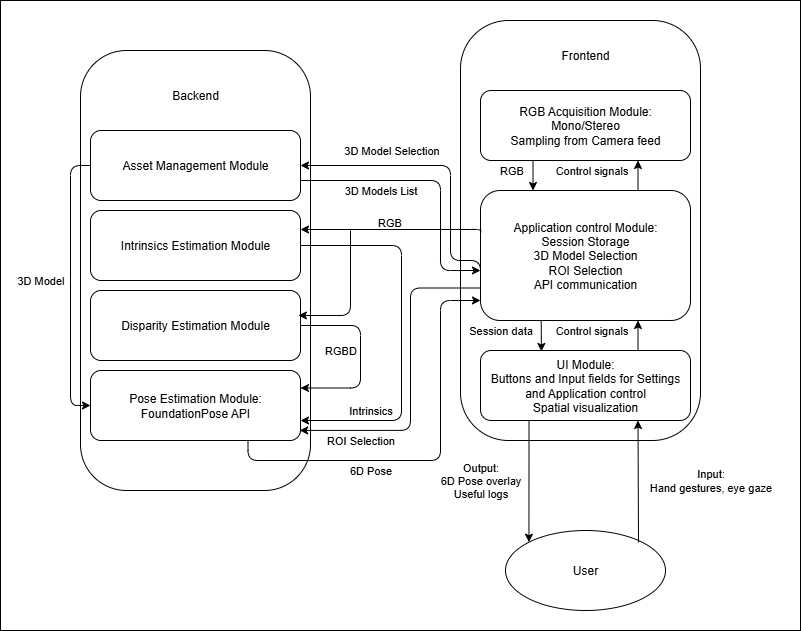
\includegraphics[width=\textwidth]{figures/AVP.png}
  \caption[High-level system architecture]{High-level system architecture: AVP UI and AirPlay mirroring, main API backend, and FoundationPose-based 6D pose estimation.}
  \label{fig:sysdesign}
\end{figure}

Early experiments attempted to stream AirPlay frames directly from \texttt{uxplay} to the pose backend. This led to visible stutter, tiling artefacts, and unstable latency. The current design centralizes AirPlay handling in the main API, which buffers frames, down-samples when necessary, and exposes diagnostics to the AVP client.

\subsection{Main API and Pose Backend}
\label{subsec:backend-api}

The main API is implemented in Python using \texttt{Flask} and runs as a long-living service. It plays two roles, summarized in Table~\ref{tab:main-api-roles}.

\begin{table}[H]
    \centering
    \caption{Main API roles}
    \label{tab:main-api-roles}
    \begin{tabular}{p{0.27\linewidth}p{0.63\linewidth}}
        \toprule
        \textbf{Role} & \textbf{Description} \\
        \midrule
        Abstraction layer &
        Provides a compact, AVP-specific endpoint (\texttt{/avp\_pose}) that hides the complexity of FoundationPose payloads. \\
        State manager &
        Maintains the latest RGB frame, intrinsics, ROI mask, depth map, and headset pose to serve both AVP and debugging tools. \\
        \bottomrule
    \end{tabular}
\end{table}

Internally, the main API forwards pose requests to the collaborator’s FoundationPose backend~\cite{matchcow_pose_api}, which is containerized with Docker and exposes a dedicated pose estimation endpoint. The FoundationPose backend expects the inputs listed in Table~\ref{tab:foundationpose-inputs} and returns homogeneous transformation matrices in $\mathrm{SE}(3)$.

\begin{table}[H]
    \centering
    \caption{Expected inputs of the FoundationPose backend}
    \label{tab:foundationpose-inputs}
    \begin{tabular}{p{0.28\linewidth}p{0.18\linewidth}p{0.44\linewidth}}
        \toprule
        \textbf{Field} & \textbf{Type} & \textbf{Description} \\
        \midrule
        Camera intrinsics & $3\times 3$ JSON & Pinhole camera matrix $K$. \\
        RGB images & PNG (base64) & One or more RGB frames. \\
        Depth maps & PNG (base64) & Depth images aligned with the RGB frames. \\
        Segmentation mask & PNG (base64) & Binary mask isolating the target object/ROI. \\
        Mesh model & PLY, base64 & 3D object model used for pose estimation. \\
        Depth scale factor & scalar (optional) & Converts depth units to metric scale if necessary. \\
        \bottomrule
    \end{tabular}
\end{table}

At startup, the FoundationPose server loads the score predictor, pose refiner, and CUDA rasterizer into GPU memory and manages memory using \texttt{torch.cuda.empty\_cache()} and \texttt{gc.collect()} to fit on 8~GB GPUs. Logs are continuously written to \texttt{pose\_api.log}.

\subsubsection{Main API Endpoint Groups}

For the AVP client and the AirPlay capture process, the main API exposes the endpoint groups summarized in Tables~\ref{tab:endpoints-health}–\ref{tab:endpoints-pose}.

\begin{table}[H]
    \centering
    \caption{Health and diagnostics endpoints}
    \label{tab:endpoints-health}
    \begin{tabular}{p{0.23\linewidth}p{0.13\linewidth}p{0.56\linewidth}}
        \toprule
        \textbf{Endpoint} & \textbf{Method} & \textbf{Purpose} \\
        \midrule
        \texttt{/health} & GET &
        Check that the server is running and reachable. \\
        \texttt{/stats} & GET &
        Return aggregated statistics (processed frames, average latency, last error message). \\
        \bottomrule
    \end{tabular}
\end{table}

\begin{table}[H]
    \centering
    \caption{Configuration and model management endpoints}
    \label{tab:endpoints-config}
    \begin{tabular}{p{0.23\linewidth}p{0.13\linewidth}p{0.56\linewidth}}
        \toprule
        \textbf{Endpoint} & \textbf{Method} & \textbf{Purpose} \\
        \midrule
        \texttt{/config} &
        GET/POST &
        Read or update configuration (HSV thresholds, depth mode, ROI defaults). \\
        \texttt{/models} & GET &
        List available \texttt{.ply} CAD models in the \texttt{models} directory. \\
        \texttt{/select\_model} & POST &
        Set the active CAD model for subsequent pose estimation calls. \\
        \bottomrule
    \end{tabular}
\end{table}

\begin{table}[H]
    \centering
    \caption{Frame, mask, depth, and intrinsics endpoints}
    \label{tab:endpoints-frame}
    \begin{tabular}{p{0.24\linewidth}p{0.11\linewidth}p{0.57\linewidth}}
        \toprule
        \textbf{Endpoint} & \textbf{Method} & \textbf{Purpose} \\
        \midrule
        \texttt{/receive\_frame} & POST &
        Ingest latest AirPlay RGB frame (base64 encoded). \\
        \texttt{/rgb\_frame} & GET &
        Retrieve the last stored RGB frame for debugging or visualization. \\
        \texttt{/mask}, \texttt{/mask\_debug} & GET &
        Return binary and debug ROI masks. \\
        \texttt{/intrinsics} & GET &
        Return the latest estimated camera intrinsics matrix $K$. \\
        \texttt{/depth}, \texttt{/disparity} & GET &
        Retrieve the current depth or disparity map. \\
        \texttt{/external\_depth} & POST &
        Inject an externally computed depth map (e.g.\ from RealSense). \\
        \bottomrule
    \end{tabular}
\end{table}

\begin{table}[H]
    \centering
    \caption{Headset pose and pose estimation endpoints}
    \label{tab:endpoints-pose}
    \begin{tabular}{p{0.24\linewidth}p{0.11\linewidth}p{0.57\linewidth}}
        \toprule
        \textbf{Endpoint} & \textbf{Method} & \textbf{Purpose} \\
        \midrule
        \texttt{/head\_pose} & POST/GET &
        Receive or query the latest headset pose (position, quaternion, timestamp). \\
        \texttt{/pose} & POST &
        Low-level pose endpoint; forwards fully assembled payloads to FoundationPose or returns mock poses. \\
        \texttt{/avp\_pose} & POST &
        High-level endpoint for AVP: accepts ROI circle parameters, color filter, depth mode, model name, and mock/real flag; reconstructs mask and depth, calls FoundationPose, optionally applies headset compensation, and returns final poses. \\
        \bottomrule
    \end{tabular}
\end{table}

The JSON payload for \texttt{/avp\_pose} is intentionally compact; the AVP never uploads full frames:

\begin{verbatim}
{
  "roi_circle": {
    "center_px": [cx, cy],
    "radius_px": r
  },
  "color_filter": {
    "h_min": ..., "h_max": ...,
    "s_min": ..., "s_max": ...,
    "v_min": ..., "v_max": ...
  },
  "depth_mode": "mde" | "realsense" | "none",
  "model_name": "banana.ply",
  "use_mock_pose": false
}
\end{verbatim}

\subsection{Computer Vision Pipeline}
\label{subsec:cv-pipeline-design}

The computer vision pipeline operates inside the main API and transforms the AirPlay RGB feed plus AVP parameters into inputs compatible with FoundationPose. The main stages are summarized in Table~\ref{tab:cv-stages}.

\begin{table}[H]
    \centering
    \caption{Computer vision pipeline stages}
    \label{tab:cv-stages}
    \begin{tabular}{p{0.24\linewidth}p{0.62\linewidth}}
        \toprule
        \textbf{Stage} & \textbf{Description} \\
        \midrule
        RGB acquisition &
        Buffer the latest AirPlay RGB frame for subsequent processing and debugging. \\
        Intrinsics estimation &
        Detect ArUco board corners and estimate camera intrinsics $K$ via OpenCV. \\
        ROI mask reconstruction &
        Rebuild a binary ROI mask using ROI circle parameters and color filtering. \\
        Depth estimation &
        Produce a depth or disparity map (monocular model or external depth sensor). \\
        Payload assembly &
        Pack RGB, depth, mask, intrinsics, and mesh into a FoundationPose request. \\
        \bottomrule
    \end{tabular}
\end{table}

A conceptual overview is shown in Figure~\ref{fig:cv_pipeline_design}.

\begin{figure}[H]
    \centering
    \fbox{\parbox{0.9\linewidth}{Placeholder: CV pipeline diagram (AirPlay RGB $\rightarrow$ intrinsics $\rightarrow$ ROI mask $\rightarrow$ depth $\rightarrow$ FoundationPose).}}
    \caption[Computer vision pipeline]{Computer vision pipeline inside the main API.}
    \label{fig:cv_pipeline_design}
\end{figure}

\subsubsection{RGB Acquisition and Intrinsics Estimation}

A capture process grabs frames from the AirPlay receiver and forwards them to \texttt{/receive\_frame}. The main API stores the most recent frame and exposes it for debugging via \texttt{/rgb\_frame}.  

Camera intrinsics $K$ are estimated by placing an ArUco marker board in the scene. The backend detects marker corners in AirPlay frames, solves a pinhole model with OpenCV, and caches the latest $K$ as long as the board is visible. This acts as a practical workaround for the missing direct access to AVP calibration data.

\subsubsection{ROI Mask Reconstruction}

The AVP client renders a circular ROI overlay into the user’s view and sends its center, radius, and color filter parameters to the backend. The backend reconstructs a pixel mask without receiving a separate mask image:

\begin{enumerate}
    \item Convert the RGB frame to HSV color space.
    \item Apply an in-range filter using the HSV bounds from the AVP to identify pixels belonging to the circle outline.
    \item Fit a circle (least-squares) to the detected outline pixels to recover center and radius in image coordinates.
    \item Fill the circle interior to obtain a binary mask (ROI = 1, background = 0).
\end{enumerate}

To avoid corrupting the RGB frame used for pose estimation, the ROI overlay in VisionOS uses a thin outline and low-opacity fill. The underlying object appearance remains visible to FoundationPose, while the outline remains detectable by color filtering.

Alternative ROI designs were explored and are summarized in Table~\ref{tab:roi-variants}.

\begin{table}[H]
    \centering
    \caption{ROI design variants evaluated during prototyping}
    \label{tab:roi-variants}
    \begin{tabular}{p{0.25\linewidth}p{0.55\linewidth}p{0.14\linewidth}}
        \toprule
        \textbf{Variant} & \textbf{Properties} & \textbf{Chosen?} \\
        \midrule
        Free-form ROI drawing &
        Arbitrary polygon or lasso selection; flexible but harder to map to gaze/gesture interaction and more complex to reconstruct on the backend. & No \\
        Active contour (snakes) on outline &
        Refines ROI boundary along image gradients; yields accurate masks but adds computational overhead unnecessary for FoundationPose. & No \\
        Circular ROI (current) &
        Simple parameterization (center, radius), easy to control via gaze + slider, cheap to reconstruct from color-coded outline. & Yes \\
        \bottomrule
    \end{tabular}
\end{table}

\subsubsection{Depth Estimation Approaches}

ADEP restrictions prevent direct use of AVP depth sensors, so several depth strategies were explored.

\paragraph*{Monocular Depth Estimation (MDE)}

An AnyDepth v2 transformer was evaluated via a HuggingFace endpoint. For each RGB frame, the backend:
\begin{enumerate}
    \item preprocesses the image to the model’s input resolution,
    \item runs inference to obtain a dense depth map,
    \item rescales the map back to the original resolution.
\end{enumerate}

Qualitative comparisons against Intel RealSense depth showed low error for typical indoor scenes, but cloud inference introduced substantial latency. In the final system, MDE is treated as an optional mode for offline testing or low-frequency updates, not as the default for interactive AR use.

\paragraph*{Multi-Camera Depth with RealSense}

To obtain metric depth while bypassing ADEP limitations, a multi-camera setup with an Intel RealSense was considered:

\begin{enumerate}
    \item Place an ArUco board visible to both RealSense and the AVP view to estimate extrinsics between the two cameras.
    \item Back-project RealSense depth into 3D, transform points into the AVP camera frame, and reproject them into the AirPlay image with Z-buffering (see Appendix~\ref{appendix:stereo}).
    \item Transform the AVP ROI mask into the RealSense frame (or vice versa) to restrict pose estimation to the target region.
\end{enumerate}

This approach increases calibration complexity but provides high-quality depth independent of AVP sensor access and supports outsourcing pose estimation to an external RGB-D camera.

\subsection{Python Prototype for Pose Estimation}
\label{subsec:python-prototype}

Due to AVP access restrictions, a separate Python desktop prototype was developed to validate the full pipeline with direct camera and depth access. Its main modules are summarized in Table~\ref{tab:python-modules}.

\begin{table}[H]
    \centering
    \caption{Core modules of the Python prototype}
    \label{tab:python-modules}
    \begin{tabular}{p{0.27\linewidth}p{0.63\linewidth}}
        \toprule
        \textbf{Module} & \textbf{Functionality} \\
        \midrule
        Model selector &
        Load PLY meshes (banana, drill, spanner, etc.), precompute geometry (center of mass, axes, edge list) for overlay. \\
        Intrinsics and ROI UI &
        Capture stereo images, send to \texttt{/intrinsics}, visualize left/right/rectified views, and allow circular ROI drawing. \\
        Depth integration &
        Integrate ZoeDepth~\cite{bhat2023zoedepth} for monocular depth maps aligned with the ROI-masked RGB. \\
        Pose integration &
        Connect either to a mock pose API or the real FoundationPose backend using the same payload format. \\
        Concurrency manager &
        Use threads and queues for snapshot, masking, and pose handling to achieve near real-time responsiveness. \\
        \bottomrule
    \end{tabular}
\end{table}

\subsubsection{3D Model Selection}

The prototype exposes a model selector that allows the user to pick a mesh from the \texttt{models} directory. Basic geometric quantities are precomputed for display, as illustrated in Figure~\ref{fig:plymodels}.

\begin{figure}[H]
  \centering
  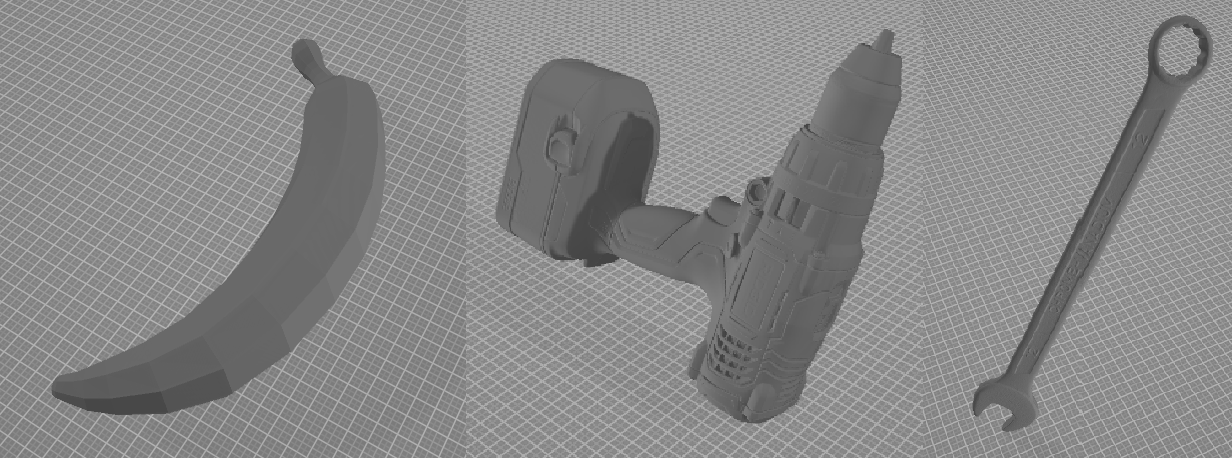
\includegraphics[width=0.8\textwidth]{figures/plymodels.png}
  \caption[Example 3D mesh models in the Python prototype]{Example 3D mesh models in the Python prototype (from left to right: banana, electric drill, spanner).}
  \label{fig:plymodels}
\end{figure}

\subsubsection{Intrinsics Estimation and ROI Selection}

The user captures left and right images from a stereo webcam and sends them to \texttt{/intrinsics}. The backend estimates $K$ and returns it. The UI displays left, right, and rectified images and provides a canvas for ROI selection (Figure~\ref{fig:pyprogramtab1}). The ROI mask is applied directly to the RGB snapshot; a preview widget confirms alignment. Early experiments with template matching for ROI tracking across frames were discarded due to instability in cluttered scenes.

\begin{figure}[H]
  \centering
  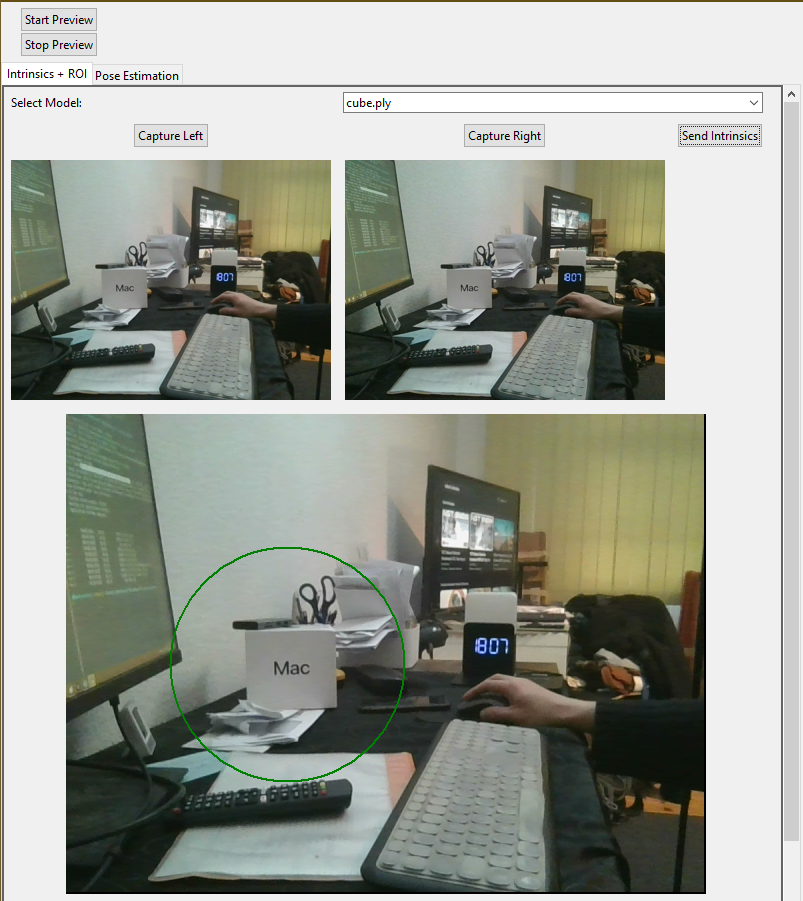
\includegraphics[width=\textwidth]{figures/basiypythonclient.png}
  \caption[Python prototype: calibration and ROI selection]{Tab~1 of the Python prototype: model selection, stereo calibration, and ROI selection.}
  \label{fig:pyprogramtab1}
\end{figure}

\subsubsection{Depth Estimation and Mock Pose API}

ZoeDepth generates dense monocular depth maps that are aligned with the ROI-masked RGB image. Figure~\ref{fig:pyprogramtab2} shows the live RGB feed, the depth map, the overlay with projected mesh and axes (using a mock pose API), and the ROI-masked input frame.

\begin{figure}[H]
  \centering
  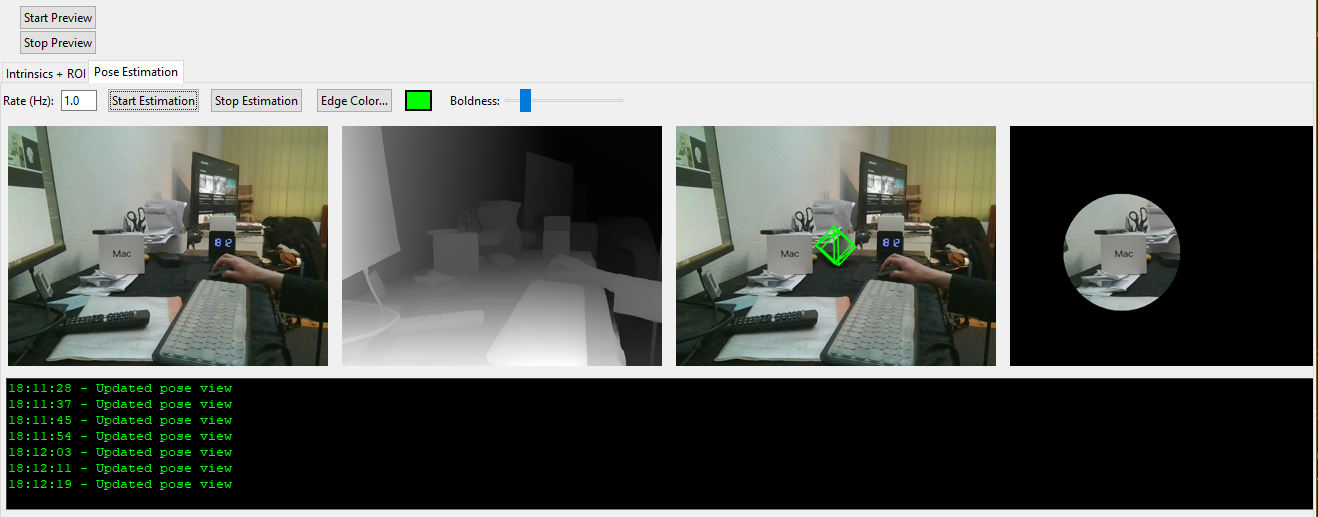
\includegraphics[width=\textwidth]{figures/basiypythonclient_2.png}
  \caption[Python prototype: depth and pose visualization]{Tab~2 of the Python prototype: live RGB feed, monocular depth map, pose overlay using a mock API, and ROI-masked input.}
  \label{fig:pyprogramtab2}
\end{figure}

The mock pose API accepts the same payloads as the real FoundationPose backend and returns plausible $\mathrm{SE}(3)$ transformations. This decouples frontend development from backend availability and accelerates testing of ROI logic and overlay visualization.

\subsubsection{Concurrency Design}

The Python client uses three queues and worker threads to decouple capture, processing, and rendering. Table~\ref{tab:python-queues} summarizes the design.

\begin{table}[H]
    \centering
    \caption{Queue-based concurrency in the Python prototype}
    \label{tab:python-queues}
    \begin{tabular}{p{0.25\linewidth}p{0.61\linewidth}}
        \toprule
        \textbf{Queue} & \textbf{Responsibility} \\
        \midrule
        Snapshot queue &
        Stores raw frames captured from the camera at maximum feasible rate. \\
        Mask/ROI queue &
        Applies circular masks, prepares RGB + depth payloads, and handles basic preprocessing. \\
        Pose queue &
        Collects API responses and forwards them to the GUI thread for overlay rendering. \\
        \bottomrule
    \end{tabular}
\end{table}

This structure informed the VisionOS concurrency design, where Swift’s \texttt{async/await} and actors replace Python threads but preserve the same conceptual separation of concerns.

\subsection{AR Interface Design on VisionOS}
\label{subsec:ar-interface-design}

The VisionOS interface is structured around three floating windows and one immersive view. Their roles are summarized in Table~\ref{tab:avp-windows}.

\begin{table}[H]
    \centering
    \caption{AVP UI components}
    \label{tab:avp-windows}
    \begin{tabular}{p{0.24\linewidth}p{0.62\linewidth}}
        \toprule
        \textbf{Component} & \textbf{Function} \\
        \midrule
        Main window &
        Configure API host and port, select CAD model, choose depth mode, and start/stop pose polling. \\
        ROI window &
        Adjust ROI circle parameters (radius slider, color picker, enable/disable toggle). \\
        Debug window &
        Display logs, diagnostic messages, last pose matrix, and approximate latency. \\
        Immersive view &
        Render the pose overlay (3D arrow) and headset pose axes in the user’s spatial environment. \\
        \bottomrule
    \end{tabular}
\end{table}

All windows are spatially repositionable. The main and ROI windows drive the configuration of the backend, while the debug window provides immediate feedback about backend behaviour and network health.

\subsubsection{ROI Interaction}

On VisionOS, ROI selection is based on gaze direction plus UI controls instead of mouse clicks. Table~\ref{tab:roi-controls} summarizes the corresponding UI elements and their backend effects.

\begin{table}[H]
    \centering
    \caption{ROI-related UI controls and backend usage}
    \label{tab:roi-controls}
    \begin{tabular}{p{0.27\linewidth}p{0.59\linewidth}}
        \toprule
        \textbf{Control} & \textbf{Effect} \\
        \midrule
        Gaze position &
        Defines the ROI circle center along a fixed depth plane in the current view. \\
        Radius slider &
        Adjusts the ROI radius in pixel coordinates; sent as \texttt{radius\_px} to the backend. \\
        Color picker &
        Sets the outline color; mapped to HSV thresholds used to detect the ROI outline in the AirPlay frame. \\
        Enable/disable toggle &
        Turns ROI-based masking on or off for the next pose request. \\
        \bottomrule
    \end{tabular}
\end{table}

The circular ROI is intentionally simpler than a free-form selection and aligns well with gaze-based interaction. It is sufficient for isolating single objects and matches the assumptions of the backend mask reconstruction.

\subsubsection{Debugging and Visualization}

The debug window displays:

\begin{itemize}
    \item the last pose matrix and a compact textual summary,
    \item approximate API round-trip time,
    \item current connection status and error messages,
    \item indicators for active depth mode and model selection.
\end{itemize}

In the immersive view, the pose is visualized as a 3D arrow aligned with the estimated object frame instead of a full CAD mesh. This keeps rendering overhead low and makes translational and rotational errors immediately visible.

\subsection{Occlusion Handling and State Estimation (Design)}
\label{subsec:occlusion-design}

The architecture anticipates occlusions and noisy pose estimates but does not yet include a full online correction module in the running system. Two complementary strategies were considered: geometric reconstruction and probabilistic filtering.

\begin{table}[H]
    \centering
    \caption{Occlusion-handling strategies considered in the design}
    \label{tab:occlusion-strategies}
    \begin{tabular}{p{0.26\linewidth}p{0.6\linewidth}}
        \toprule
        \textbf{Strategy} & \textbf{Idea} \\
        \midrule
        Geometric methods &
        Use multi-camera setups (RealSense + AVP), 3D reconstruction from multiple views, and depth-based occlusion reasoning (nearest-surface logic) to explicitly model visibility. \\
        Probabilistic state estimation &
        Model the object pose as a hidden state driven by headset motion and noisy pose measurements, and use filters (EKF, PF, GP-based models) to smooth and correct poses under occlusions. \\
        \bottomrule
    \end{tabular}
\end{table}

In the probabilistic case, the filters operate solely on:

\begin{itemize}
    \item the stream of noisy object poses estimated by FoundationPose, and
    \item the headset pose stream obtained from VisionOS.
\end{itemize}

User input (gestures, configuration changes) does not enter the mathematical model. EKF and PF formulations are sketched in Section~\ref{subsec:occlusion-design}, and a data-driven approach based on Willems’ Fundamental Lemma combined with Gaussian Process residual correction is described in Appendix~\ref{appendix:willems}. Simulation results suggest improved robustness under intermittent occlusions and slowly drifting intrinsics compared to a baseline EKF. Integrating such a module into the online AVP pipeline is left as future work.

Overall, the system design enforces a clear separation between sensing (via AirPlay and headset tracking), backend processing (intrinsics, masking, depth, pose), and AR visualization, while keeping the architecture open to more advanced occlusion handling and state estimation techniques in subsequent iterations.
